\documentclass{beamer}
%pacchetti
\usepackage[T1]{fontenc}
\usepackage[utf8]{inputenc}
\usepackage{graphicx}
\usepackage[italian]{babel}
\usepackage{mathrsfs}
\usepackage{booktabs}
\usepackage{amsmath}
\usepackage{amsfonts}
\usepackage{amssymb}
\usepackage{amsbsy}
\usepackage{amsthm}
\usepackage{enumerate}
\usepackage{quoting}
\quotingsetup{font=small}
\usepackage{diagbox}
\usepackage{graphicx}
\usepackage{setspace}
\usepackage{float}
\usepackage{version}
\usepackage{multicol}
\usepackage{beamerfoils}

\usepackage[none]{hyphenat} %avoid hyphenation
\usepackage{xcolor} %to uset \textcolor
\usepackage{bbm} %funzione indicatrice
% end pacchetti

\usetheme[bgphoto]{polimi}

% Full instructions available at:
% https://github.com/elauksap/beamerthemepolimi

% Set custom font (requires to compile with XeLaTeX).
\usepackage{ifxetex}
\ifxetex
\usepackage{fontspec}
\setsansfont[Scale=0.9]{Arial}
\fi

\usepackage{lipsum}


\newcommand\mynum[1]{%
	\usebeamercolor{enumerate item}%
	\tikzset{beameritem/.style={circle,inner sep=0,minimum size=2ex,text=enumerate item.bg,fill=enumerate item.fg,font=\footnotesize}}%
	\tikz[baseline=(n.base)]\node(n)[beameritem]{#1};%
}


\title{Coupled Markov chains with applications to Approximate Bayesian Computation for model based clustering}
%\subtitle{Subtitle}
\author{E. Bertoni, M. Caldarini, F. Di Filippo, G. Gabrielli, E. Musiari}
\date{10 January 2022}


%Cose da fare

% Mettere biografia
% Mettere \pause e colori
% Sistemare il titolo e layout

\begin{document}

\begin{frame}
\maketitle
\end{frame}

	
\begin{section}{Introduction}

	\begin{frame}
		\frametitle{A complex problem}

 		\begin{minipage}{0.45\textwidth}
 			\begin{center}
 				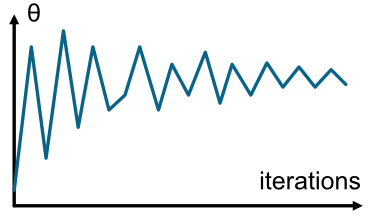
\includegraphics{img/markov_singola}
 			\end{center}
 		\end{minipage}
 		\hfill
 	 	\begin{minipage}{0.45\textwidth}
 	 		\begin{center}
 	 				
\includegraphics{img/likelihood_na}
 	 		\end{center}
 		\end{minipage}
 		
 		\vspace{0.5cm}

 		\begin{minipage}{0.45\textwidth}
 			\begin{center}
 				$\Downarrow$

 				\textbf{Unbiased Markov chain Monte Carlo methods with couplings}
 			\end{center}
 		\end{minipage} %}
 		\hfill
	 	\begin{minipage}{0.45\textwidth}
 			\begin{center}
 				$\Downarrow$
 				
 				 \textbf{Approximate Bayesian Computation}
 			\end{center}
 		\end{minipage} %}
 	 	
 	 	\vspace{0.2cm}
 	 	
 	 	\begin{minipage}{0.45\textwidth}
 	 		\begin{center}
 	 			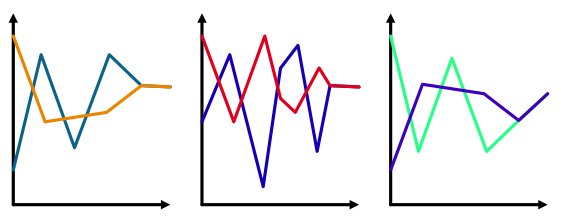
\includegraphics{img/markov_coupled_parallel}
 	 		\end{center}
 	 	\end{minipage}%}
 	 	\hfill
 	 	\begin{minipage}{0.45\textwidth}

 	 	\end{minipage}
 	 	
 	 	
 	 	
	\end{frame}

\end{section}
	
	
\begin{section}{Approximate Bayesian Computation}
	
	\begin{frame}[plain]{}
	\sectionpage
\end{frame}

%%%% (dire quale summary statistica usata, quale distanza usata, quale kernel)
\begin{frame}{ABC Metropolis Hastings}
\only<1,2,4,5,7> {
	\emph{Inputs:}
	\begin{itemize}
		\item a target posterior density $\pi(\theta | y_{obs}) \propto p(y_{obs}|\theta) \pi(\theta)$, consisting of a prior distribution $\pi(\theta)$ and a procedure of generating data under the model $p(y_{obs}|\theta)$;
		\item a Markov proposal density $g(\theta,\theta')$=$g(\theta' | \theta)$;
		\item an integer $N \textgreater0$;
		\only<1,4,5,7>{\item a kernel function $K_h(u)$ and a scale parameter $h > 0$;}
		\only<2>{\item  \textcolor{orange}{a kernel function $K_h(u)$ and a scale parameter $h > 0$};}
		\only<1,2,4,7>{\item a low dimensional vector of summary statistics $s=S(y)$.}
		\only<5>{\item \textcolor{orange}{a low dimensional vector of summary statistics $s=S(y)$}.}
	\end{itemize}
	
	\emph{Initialise:} \\
	repeat:
	\begin{enumerate}
		\item choose an initial parameter vector $\theta^{(0)}$ from the support of $\pi(\theta)$;
		\item generate $ y^{(0)} \sim p(y|\theta ^ {(0)})$ from the model and compute summary statistics $s^{(0)}=S(y^{(0)})$, until ${K_h(\parallel s^{(0)}-s_{obs}\parallel)} >0$.
	\end{enumerate}
}

\only<3> {

\begin{itemize}
	\item  a kernel function $K_h(u)$ and a scale parameter $h > 0$:
\end{itemize}

 
 $$\pi(\theta, y| y_{obs}) \propto \textcolor{orange}{\mathbbm{1}(\parallel y-y_{obs} \parallel \leq h)}p(y|\theta)\pi(\theta)$$
 \[ \Downarrow \]
 \[		\pi_{ABC}(\theta, y | y_{obs}) \propto \textcolor{orange}{K_h(u)}p(y|\theta)\pi(\theta)\]
 
 
 \vspace{0.7cm}
 Where $K$ is a standard smoothing kernel function and:
 \[ \textcolor{orange}{K_h(u)}  =  \frac{1}{h}  K \left( \frac{u}{h} \right), \quad \text{ with } \  u=\parallel y-y_{obs} \parallel \]
 
 

}

\only<6>{
	
	\begin{itemize}
		\item a low dimensional vector of summary statistics $s=S(y)$:
	\end{itemize}

\vspace{0.5cm}
	 $$ K_h(\parallel  y-y_{obs} \parallel ) $$
	\[ \Downarrow \]
	\[	K_h(\parallel S(y) - S(y_{obs}) \parallel )	\]
	

}

\only<8> {
	\emph{Sampling} for $i=1,...,N$:
	\begin{enumerate}
		\item generate candidate vector $\theta' \sim g(\theta^{(i-1)},\theta)$ from the proposal density $g$;
		\item generate $ y\,' \sim p(y|\theta')$ from the model and compute summary statistics  $s' = S(y\,')$;
		\item with probability $$\min \{ 1, \frac{K_h(\parallel s'-s_{obs}\parallel)   \pi(\theta')g(\theta',\theta^{(i-1)})}{K_h(\parallel s^{(i-1)}-s_{obs}\parallel)   \pi(\theta^{(i-1)})g(\theta^{(i-1)},\theta') } \}$$ 
		set $(\theta^{(i)},s^{(i)})=(	\theta',s')$. 
		Otherwise set  $(\theta^{(i)},s^{(i)})=(\theta^{(i-1)},s^{(i-1)})$.
	\end{enumerate}
	
	\emph{Output:}
	\begin{itemize}
		\item a set of correlated parameter vectors $\theta ^ {(1)},..., \theta ^ {(N)}$ from a Markov chain with stationary distribution $\pi_{ABC}(\theta |S_{obs})$.
	\end{itemize}
}
\end{frame}



\begin{frame}
\frametitle{Study case}
\only<1>{
\textbf{Summary statistic}: \\
\begin{center}
	Sample mean, vector of 9 quantiles
\end{center}

\textbf{Distance}: 
\begin{center}
	2-norm of the difference
\end{center}   %malanobis nel multivariato

\textbf{Kernel}: 
$$
K(u) = 
\frac{1}{\sqrt{2\pi}} e^{-\frac{1}{2}u^2}, 
\quad K_h(u) 
= \frac{K(\frac u h)}{h}
$$
%1/(np.sqrt(2*math.pi))np.exp(-1/2*u*2)
}
\only<2>{

\begin{block}{Model}
	\begin{center}
		$ Y_i | \mu \overset{iid}{\sim} \mathcal{N}(\mu, \sigma_{obs} ^2) $\\
		
		\vspace{0.3cm}
		
		$ \mu  \sim \mathcal{N}(\mu_0, \sigma_0^2)$
		
		$\mu_0 = 8, \quad \sigma^2_0 = 4$
	\end{center}
\end{block}

\begin{block}{Dataset}
	100 samples generated from a Gaussian distribution:
	\begin{center}
		$
		Y_{obs} \sim \mathcal{N}(\mu_{obs}, \sigma_{obs} ^2)
		$
		
		$
		\mu_{obs} = 10, \quad
		\sigma_{obs} ^2 = 3
		$
	\end{center}
\end{block}
}
\end{frame}


\begin{frame}{Results}

	{\small
		\textbf{Posterior distribution:}
		
		$$
		\mathcal{N}(\mu_n, \sigma^2_n), 
		\vspace{0.3cm}
		%\quad
		\mu_n 
		= \frac{1}{ \frac{1}{\sigma_0^2} + \frac{n}{\sigma_{obs}^2} } 
		\cdot \left(\frac{\mu_0}{\sigma_0^2} + \frac{\sum y_{obs}}{\sigma_{obs}^2}\right)
		\simeq 10.151,
		\vspace{0.3cm}
		%\quad
		\sigma^2_n
		= \frac{1}{ \frac{1}{\sigma_0^2} + \frac{n}{\sigma_{obs}^2} } 
		\simeq 0.0298
		$$
	}



\begin{minipage}{0.45\textwidth}
\begin{center}
	{\scriptsize \textbf{Sampling}}
	\includegraphics[width=\textwidth]{}
\end{center}
\end{minipage}
\hfill
\begin{minipage}{0.45\textwidth}
\begin{center}
	{\scriptsize \textbf{Sampling histogram with real distribution}}
	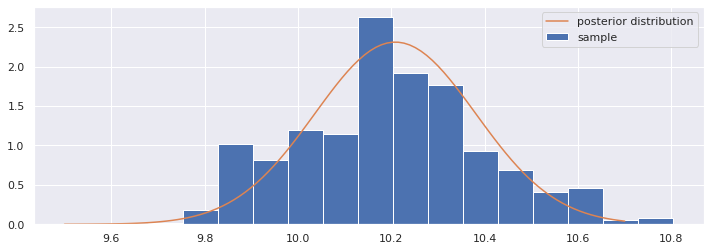
\includegraphics[width=\textwidth]{ABC_graphs/ABCunivgraphic}
\end{center}
\end{minipage}


\end{frame}


\begin{frame}{Results}
The same model using as summary statistic a vector of 9 quantiles:
\begin{center}
	\begin{minipage}{0.63\textwidth}
		\begin{center}
			{\scriptsize \textbf{Sampling}}
			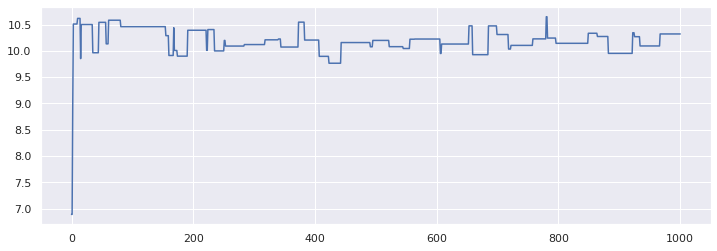
\includegraphics[width=\textwidth]{ABC_graphs/ABC_S1_1000iter}
		\end{center}
	\end{minipage}
	
	\vspace{0.2cm}
	
	\begin{minipage}{0.63\textwidth}
		\begin{center}
			{\scriptsize \textbf{Sampling histogram with real distribution}}
			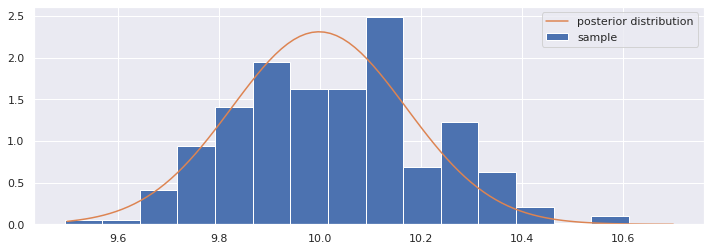
\includegraphics[width=\textwidth]{ABC_graphs/ABC_S1}
		\end{center}
	\end{minipage}
\end{center}
% grafici per un esempio univariato con summary mean -> e uno con quantili? (funzionava?)
\end{frame}


\end{section}
	
	\begin{section}{Conclusions}
	
    \begin{frame}[plain]{}
		\sectionpage
	\end{frame}

	\begin{frame}{Next steps}
	
		The next step will be the conclusion of the implementation of the MCMC with couplings and approximate bayesian computation on multivariate data.
		
		\vspace{0.5 cm}
		Further steps will be implementing the version with unknown variance and testing on more complex data.
		
		Finally, making comparisons with a standard MCMC algorithm.
	\end{frame}

	\begin{frame}{Bibliography}
		\nocite{*}
		\bibliographystyle{unsrt}
		\tiny{ \bibliography{refs_MCMC,refs_ABC} }

	
%				\begin{minipage}[t]{0.4\textwidth}
%			\footnotesize {Unbiased Markov chain Monte Carlo methods with couplings:}
%			\tiny { \bibliography{refs_MCMC} }
%		\end{minipage}
%		\hfill
%		\begin{minipage}[t]{0.4\textwidth}
%			\footnotesize {Approximate Bayesian computation:}
%			\tiny { \bibliography{refs_ABC} }
%		\end{minipage}

	\end{frame}
\end{section}

%------------------------------------------------------------------------------------	
\begin{frame}
	\frametitle{Metropolis Hastings with couplings and ABC}
	\only<1>{
		\begin{enumerate}
			\item Compute $s_{obs} = S(y_{obs})$;
			\item generate $\mu_{x}^{(0)} \sim  \pi(\mu)$ and $\mu_{y}^{(0)} \sim  \pi(\mu)$ from prior density;
			\item generate $\sigma_{x}^{2(0)} \sim  \pi(\sigma^2)$ and $\mu_{y}^{2(0)} \sim  \pi(\sigma^2)$ from prior density;
			\item generate with a maximal coupling two samples of N observations such that $y_{1i} \sim \mathcal{N}(\mu_{x}^{(0)}, \sigma_{x}^{2(0)})$ and  $y_{2j} \sim \mathcal{N}(\mu_{y}^{(0)},\sigma_{y}^{2(0)})$;
			\item compute $s_{x}^{(0)}=S(y_{1})$ and $s_{y}^{(0)}=S(y_{2})$;
			\item until $K_h(||s_{x}^{(0)}-s_{obs}||)>0$:
			\begin{itemize}
				\item generate $\mu_{x}^{(0)} \sim  \pi(\mu)$ and $\sigma_{x}^{2(0)} \sim  \pi(\sigma^2)$ from prior densities;
				%	\item generate $\sigma_{x}^{2(0)} \sim  \pi(\sigma^2)$ from prior density;
				\item generate a sample of N observations such that $y_{1i} \sim \mathcal{N}(\mu_{x}^{(0)},\sigma_{x}^{2(0)})$;
				\item compute $s_{x}^{(0)}=S(y_{1})$;
			\end{itemize}
			\item until $K_h(||s_{y}^{(0)}-s_{obs}||)>0$:
			\begin{itemize}
				\item generate $\mu_{y}^{(0)} \sim  \pi(\mu)$ and $\sigma_{y}^{2(0)} \sim  \pi(\sigma^2)$  from prior densities;
				% generate $\sigma_{y}^{2(0)} \sim  \pi(\sigma^2)$ from prior density;
				\item generate a sample of N observations such that $y_{1i} \sim \mathcal{N}(\mu_{y}^{(0)},\sigma_{y}^{2(0)})$;
				\item compute $s_{x}^{(0)}=S(y_{1})$;
			\end{itemize}
			
		\end{enumerate}
	}
	\only<2>{
		\begin{enumerate}
			\setcounter{enumi}{7}	
			
			\item for i = 1,...,N:
			given $$\theta^{(i-1)}=(\mu^{(i-1)},\sigma^{2(i-1)})$$
			\begin{itemize}
				
				\item generate [$\theta_{x}^{(i)},\theta_{y}^{(i)}$] from a maximal coupling given [$\theta_{x}^{(i-1)},\theta_{y}^{(i-1)}$];
				\item generate from a maximal coupling two samples of N observations $y_{1} \sim p(y|\theta_{x}^{(i)})$ and $y_{2} \sim p(y|\theta_{y}^{(i)})$;
				\item compute $s_{x}^{(i)}=S(y_{1})$ and $s_{y}^{(i)}=S(y_{2})$;
				\item accept $\theta_{x}^{(i)}$ with probability 
				$$
				\frac{
					K_h(||s_{x}^{(i)}-s_{obs}||)\pi(\theta_{x}^{(i)})
				}{
					K_h(||s_{x}^{(i-1)}-s_{obs}||)\pi(\theta_{x}^{(i-1)})
				}
				$$
				and accept $\theta_{y}^{(i)}$ with probability
				$$
				\frac{
					K_h(||s_{y}^{(i)}-s_{obs}||)\pi(\theta_{y}^{(i)})
				}{
					K_h(||s_{y}^{(i-1)}-s_{obs}||)\pi(\theta_{y}^{(i-1)})
				}.
				$$ 
			\end{itemize}
			
			
		\end{enumerate}
	}
	\only<3>{
		As output we get two sets of parameter vectors: 
		
		$$\mu_{x}^{(1)},...,\mu_{x}^{(N)}\sim \pi_{ABC} (\mu|y_{obs});$$
		$$\mu_{y}^{(1)},...,\mu_{y}^{(N)} \sim \pi_{ABC} (\mu|y_{obs}).$$
		
		$$\sigma_{x}^{2(1)},...,\sigma_{x}^{2(N)}\sim \pi_{ABC} (\sigma^2|y_{obs});$$
		$$\sigma_{y}^{2(1)},...,\sigma_{y}^{2(N)} \sim \pi_{ABC} (\sigma^2|y_{obs}).$$
		
	}
	
	
\end{frame}
%------------------------------------------------------------------------------------
\begin{frame}
	\frametitle{Maximal coupling of both parameters }
	Set $p = \mathcal{N}(X_{t-1},0.1^2*\mathbb{I})$ and $q = \mathcal{N}(Y_{t-1},0.1^2*\mathbb{I})$, then:
	\begin{enumerate}
		\item sample $X_t \sim p$;
		\item sample $W|X_t \sim \mathcal{U}\{[0,p(X_t)]\}$;
		\item if $W\leq q(X_t)$ then output $(X_t,X_t)$, otherwise:
		\begin{enumerate}
			\item sample $Y_t \sim q$;
			\item sample $W^\star | Y_t \sim \mathcal{U}\{[0, q(Y_t)]\}$ 
			until $W^\star > p(Y_t)$ and output $(X_t,Y_t)$.
		\end{enumerate}
	\end{enumerate}
\end{frame}

\begin{frame}
	\frametitle{Study case}
	
	\textbf{Summary statistic}: \\
	\begin{center}
		Sample mean, Sample Variance
	\end{center}
	
	\textbf{Distance}: 
	\begin{center}
		$$L^2-norm\ of\ the\ difference\ of\ S(y)\ and\ s_{obs}$$
	\end{center}   %malanobis nel multivariato
	
	\textbf{Kernel}: 
	$$
	K(u) = 
	\frac{1}{\sqrt{2\pi}} e^{-\frac{1}{2}u^2}, 
	\quad K_h(u) 
	= \frac{K(\frac u h)}{h}
	$$
	%1/(np.sqrt(2*math.pi))np.exp(-1/2*u*2)
	
\end{frame}

\begin{frame}
	
	\begin{block}{Model}
		\begin{center}
			
			$$ Y_i | \mu, \sigma^2 \overset{iid}{\sim} \mathcal{N}(\mu, \sigma^2) $$
			$$ \mu  \sim \mathcal{N}(\mu_0, \sigma_0^2)  $$
			$$ \sigma^2  \sim InvGa(a,b) $$
			$$ \pi( \mu,\sigma) =\pi(\mu)*\pi(\sigma) $$
			$$ \mu_0 = 34, \quad \sigma^2_0 = 3$$
			$$ a=b=1 $$
			
		\end{center}
	\end{block}
	
\end{frame}

\begin{frame}
	\begin{block}{Dataset}
		100 samples generated from a Gaussian distribution:
		\begin{center}
			$$ Y_{obs} \sim \mathcal{N}(\mu_{obs}, \sigma_{obs}^{2}) $$
			$$	\mu_{obs} = 30,	\sigma_{obs}^{2} = 2	$$
		\end{center}
	\end{block}
	
\end{frame}



\begin{frame}
	\frametitle{Results}
	$ E[\mu|y]=30,19 $
	\begin{center}
		\begin{minipage}{0.63\textwidth}
			\begin{center}
				{\scriptsize \textbf{Coupled chains}}
				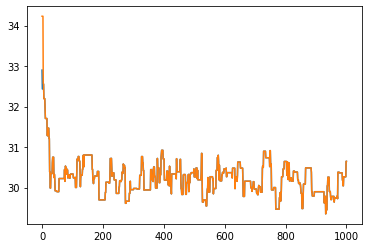
\includegraphics[width=6cm,height=3cm]{immagini_mario/mu_chains}
			\end{center}
		\end{minipage}
		
		\vspace{0.2cm}
		
		\begin{minipage}{0.63\textwidth}
			\begin{center}
				{\scriptsize \textbf{Sampling histogram with real distribution}}
				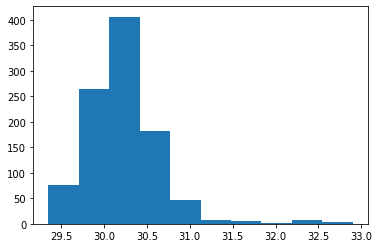
\includegraphics[width=6cm,height=3cm]{immagini_mario/mu_hist}
			\end{center}
		\end{minipage}
	\end{center}
\end{frame}

\begin{frame}
	\frametitle{Results}
	$ E[\sigma^2|y]=2,06 $
	\begin{center}
		\begin{minipage}{0.63\textwidth}
			\begin{center}
				{\scriptsize \textbf{Coupled chains}}
				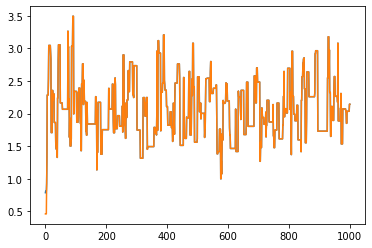
\includegraphics[width=6cm,height=3cm]{immagini_mario/sigma_chains}
			\end{center}
		\end{minipage}
		
		\vspace{0.2cm}
		
		\begin{minipage}{0.63\textwidth}
			\begin{center}
				{\scriptsize \textbf{Sampling histogram with real distribution}}
				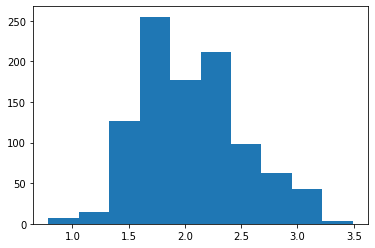
\includegraphics[width=6cm,height=3cm]{immagini_mario/sigma_hist}
			\end{center}
		\end{minipage}
	\end{center}
\end{frame}

\end{section}
%%%%%%%%%%%%%%%%%%%%%%%%%%%%%%%%%%%%%%%%%%%%%%%%%%%%%%%%%%%%%%%%%%%%%%%%%%%%%%%%%%%%%%%%%%%%%%%
\begin{section}{Numerical experiment: g-and-k distribution}
\begin{frame}
	\frametitle{Model}
	\begin{block}{QUANTILE FUNCTION:}
		
		$$ r \in (0,1) \longmapsto   a + b (1+0.8\left(\frac{1-exp(-g \cdot z(r))}{1+exp(-g\cdot z(r))}\right)(1+ z(r)^{2})^k\cdot z(r)  $$
	\end{block}	
	where $$ z(r)$$ is the r-th quantile of the standard Normal distribution. 
	\begin{block}{Model}
		Prior distribution:
		$ a \sim \mathcal{U}([0,10])$
		
		$ b \sim \mathcal{U}([0,10])$
		
		$ g \sim \mathcal{U}([0,10])$
		
		$ k \sim \mathcal{U}([0,10])$
	\end{block}
\end{frame}



\begin{frame}
	\frametitle{Study case}
	
	\textbf{Summary statistic}: \\
	\begin{center}
		10 quantile + minimum
	\end{center}
	
	\textbf{Distance}: 
	\begin{center}
		$$L^2-norm\ of\ the\ difference\ of\ S(y)\ and\ s_{obs}$$
	\end{center}   %malanobis nel multivariato
	
	\textbf{Kernel}: 
	$$
	K(u) = 
	\frac{1}{\sqrt{2\pi}} e^{-\frac{1}{2}u^2}, 
	\quad K_h(u) 
	= \frac{K(\frac u h)}{h}
	$$
	%1/(np.sqrt(2*math.pi))np.exp(-1/2*u*2)
	
\end{frame}


\begin{frame}
	\frametitle{Study case}
	\begin{block}{Dataset}
		100 samples generated from the quantile distribution:
		\begin{center}
			$$a_{obs}= 3, \ b_{obs}= 1, \ g_{obs}=2 , \ k_{obs}=0.5, \ y_{obs}$$
			$$	y_{obs} =a_{obs} + b_{obs} (1+0.8\left(\frac{1-exp(-g_{obs}\cdot z(r))}{1+exp(-g_{obs}\cdot z(r))}\right)(1+z(r)^{2})^k\cdot z(r)	$$
			and $$ z(r) \overset{iid}{\sim} \mathcal{N}(0,1) $$
		\end{center}
	\end{block}
	
\end{frame}

\begin{frame}
	\frametitle{ABC ALGORITHM}
	
	INITIALIZATION:
	
	$\theta^{(0)}=(a^{(0)},b^{(0)},g^{(0)},k^{(0)})$
	
	$ \theta^{(0)} \sim \mathcal{U}([0,10]^{4})$
	
	for j in (1,...,n):
	
	\begin{itemize}
		\item $z^{(0,j)}(r) \sim \mathcal{N}(0,1)  $
		
		\item $ y^{(0,j)} \sim quantile function(z^{(0,j)}(r))$
	\end{itemize}
	compute the summaries statistics:
	$ s^{(0)} =S(y^{(0)})$
	
	Untill $Kh(\|s^{(0)}-s_{obs}\|)>0$
	\begin{itemize}
		\item Generate $\theta^{(0)} \sim \mathcal{U}([0,10]^{4})$ from prior density.
		\item Generate $z^{(0)}(r) \sim \mathcal{N}(0,1)$
		\item Generate a sample of 1000 observations such that $y \sim quantile function(z^{(0)}(r),\theta^{(0)})$
		\item Compute $s^{(0)}=S(y)$
	\end{itemize}
	
\end{frame}

\begin{frame}
	\frametitle{ABC ALGORITHM}
	
	
	for i in (1,...,M):
	\begin{enumerate}
		\item given $\theta^{(i-1)}=(a^{(i-1)},b^{(i-1)},g^{(i-1)},k^{(i-1)})$
		
		$\theta^{(i)} \sim \mathcal{N}(\theta^{(i-1)},I)$
		
		for j in (1,...,n):
		
		$z^{(i,j)}(r) \sim \mathcal{N}(0,1)$
		
		$ y^{(ij)} \sim quantile function(z^{(i,j)}(r), \theta^{(i-1)})$
		
		
		\item Compute the summaries  $ s^{(i)} =S(y^{(i)})$
		
		\item Accept $\theta^{(i)}$ with probability $\frac{Kh(\|s^{(i)}-s_{obs}\|)\pi(\theta^{(i)})}{Kh(\|s^{(i-1)}-s_{obs}\|)\pi(\theta^{(i-1)})}$
		
	\end{enumerate} 
\end{frame}




\begin{frame}
	\frametitle{ABC + COUPLED MARKOV CHAIN for parameter a}
	
	parameters b,g,k are fixed equal to the observation parameters
	
	
	$ a_{1}^{(0)} \sim \mathcal{U}([0,10])$
	
	$ a_{2}^{(0)} \sim \mathcal{U}([0,10])$
	
	for j in (1,...,$n_{obs}$):
	\begin{itemize}
		\item $z^{(0,j)}(r) \sim \mathcal{N}(0,1)  $
		
		\item $ y_{1}^{(0,j)} \sim quantile function(z^{(0,j)}(r))$
		
		\item compute $ s_{1}^{(0)} =S(y_{1}^{(0)})$
	\end{itemize}
	for j in (1,...,$n_{obs}$):
	
	\begin{itemize}
		\item $z^{(0,j)}(r) \sim \mathcal{N}(0,1)  $
		
		\item $ y_{2}^{(0,j)} \sim quantile function(z^{(0,j)}(r))$
		
		\item compute the summaries statistics:
		$ s_{2}^{(0)} =S(y_{2}^{(0)})$
	\end{itemize}
	
\end{frame}
\begin{frame}
	\frametitle{ABC + COUPLED MARKOV CHAIN for parameter a}
	Untill $Kh(\|s_{1}^{(0)} - s_{obs}\|)>0$:
	\begin{enumerate}
		\item Generate $a_{1}^{(0)} \sim \mathcal{U}([0,10])$ from prior density.
		\item Generate $z_{1}^{(0)}(r) \sim \mathcal{N}(0,1)$
		\item Generate a sample of 1000 observations such that $y_{1} \sim quantile function(z_{1}^{(0)}(r),a_{1}^{0})$
		\item Compute $s_{1}^{(0)}=S(y_{1})$
		
	\end{enumerate}
	Untill $Kh(\|s_{2}^{(0)} - s_{obs}\|)>0$:
	\begin{enumerate}
		\item Generate $a_{2}^{(0)} \sim \mathcal{U}([0,10])$ from prior density.
		\item Generate $z_{2}^{(0)}(r) \sim \mathcal{N}(0,1)$
		\item Generate a sample of 1000 observations such that $y_{2} \sim quantile function(z_{2}^{(0)}(r),a_{2}^{(0)})$
		\item Compute $s_{2}^{(0)}=S(y_{2})$
	\end{enumerate}
	
\end{frame}
\begin{frame}
	\frametitle{ABC + COUPLED MARKOV CHAINS for parameter a}
	for i in (1,...,M):
	\begin{enumerate}
		\item 	generate $a_{1}^{(i)},a_{2}^{(i)}$  from maximalcoupling$(a_{1}^{(i-1)},a_{2}^{(i-1)})$
		
		\begin{block}
			
			for j in (1,...,n):
			\begin{itemize}
				\item $z^{(i,j)}(r) \sim \mathcal{N}(0,1)$
				\item generate:
				$ y_{1}^{(ij)} \sim quantile function(z^{(i,j)}(r), \theta^{(i-1)})$
				$ y_{2}^{(ij)} \sim quantile function(z^{(i,j)}(r), \theta^{(i-1)})$
				
			\end{itemize}
		\end{block}
		\item Compute the summaries  $ s_{1}^{(i)} =S(y_{1}^{(i)})$ and $ s_{2}^{(i)} =S(y_{2}^{(i)})$
		
		
		\item acceptance:
		\begin{itemize}
			\item Accept $a_{1}^{(i)}$ with probability $\frac{Kh(\|s_{1}^{(i)}-s_{obs}\|)\pi(a_{1}^{(i)})}{Kh(\|s_{1}^{(i-1)}- s_{obs}\|)\pi(a_{1}^{(i-1)})} $   otherwise $a_{1}^{(i)}=a_{1}^{(i-1)}$
			
			\item Accept $a_{2}^{(i)}$ with probability $\frac{Kh(\|s_{2}^{(i)}-s_{obs}\|)\pi(a_{2}^{(i)})}{Kh(\|s_{2}^{(i-1)}-s_{obs}\|)\pi(a_{2}^{(i-1)})} $  otherwise $  a_{2}^{(i)}=a_{2}^{(i-1)}$
		\end{itemize}
	\end{enumerate}
\end{frame}

\begin{frame}
	\frametitle{Maximal coupling}
	given  $(a_{1}^{(i-1)}, \ a_{2}^{(i-1)})$
	
	set	$p( \cdot |a_{1}^{(i-1)})= \mathcal{N}(a_{1}^{(i-1)},1)$ and $q( \cdot |a_{2}^{(i-1)})= \mathcal{N}(a_{2}^{(i-1)},1)$
	\begin{enumerate}
		\item $ a_{1}' \sim p( \cdot |a_{1}^{(i-1)} ) $
		
		\item if $ w_{1}\sim \mathcal{U}((0, p(a'|a_{1}^{(i-1)}))) < q(a'|a_{2}^{(i-1)} ): a_{1}^{(i)}=a_{1}' \ and \ a_{2}^{(i)}= a_{1}'$
	\end{enumerate}
	otherwise until $ w_{2}\sim \mathcal{U}((0, q(a'|a_{2}^{(i-1)})) > p(a'|a_{1}^{(i-1)} )$:
	
	\begin{enumerate}
		\item generate $ a_{2}' \sim q( \cdot |a_{2}^{(i-1)} ) $
		
		\item sample $ l \sim \mathcal{U}((0,1)) $
	\end{enumerate}
	and then set:   $ \ a_{1}^{(i)}=a_{1}' \ and \ a_{2}^{(i)}= a_{2}'$
	
	
\end{frame}


\begin{frame}
	\frametitle{Results: parameter a}
	\begin{center}
		\begin{minipage}{0.63\textwidth}
			\begin{center}
				{\scriptsize \textbf{Coupled chains}}
				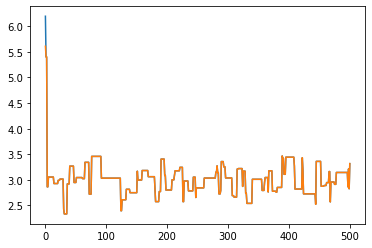
\includegraphics[width=6cm,height=3cm]{immagini_mario/a_chains}
			\end{center}
		\end{minipage}
		
		\vspace{0.2cm}
		
		\begin{minipage}{0.63\textwidth}
			\begin{center}
				{\scriptsize \textbf{Sampling histogram with real distribution}}
				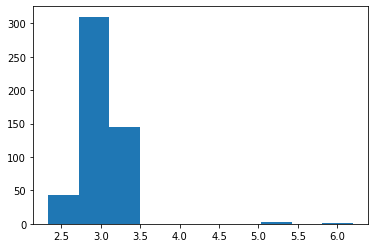
\includegraphics[width=6cm,height=3cm]{immagini_mario/a_hist}
			\end{center}
		\end{minipage}
	\end{center}
\end{frame}

\begin{frame}
	\frametitle{Results: parameter b}
	\begin{center}
		\begin{minipage}{0.63\textwidth}
			\begin{center}
				{\scriptsize \textbf{Coupled chains}}
				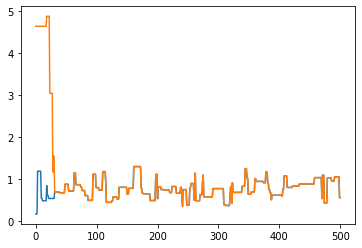
\includegraphics[width=6cm,height=3cm]{immagini_mario/b_chains}
			\end{center}
		\end{minipage}
		
		\vspace{0.2cm}
		
		\begin{minipage}{0.63\textwidth}
			\begin{center}
				{\scriptsize \textbf{Sampling histogram }}
				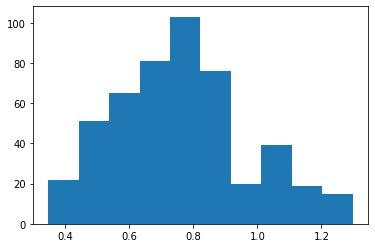
\includegraphics[width=6cm,height=3cm]{immagini_mario/b_hist}
			\end{center}
		\end{minipage}
	\end{center}
\end{frame}
\begin{frame}
	\frametitle{Results: parameter g}
	\begin{center}
		\begin{minipage}{0.63\textwidth}
			\begin{center}
				{\scriptsize \textbf{Coupled chains}}
				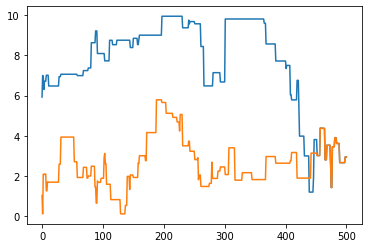
\includegraphics[width=6cm,height=3cm]{immagini_mario/g_chains}
			\end{center}
		\end{minipage}
		
		\vspace{0.2cm}
		
		\begin{minipage}{0.63\textwidth}
			\begin{center}
				{\scriptsize \textbf{Sampling histogram }}
				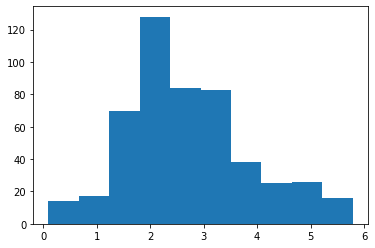
\includegraphics[width=6cm,height=3cm]{immagini_mario/g_hist}
			\end{center}
		\end{minipage}
	\end{center}
\end{frame}
\begin{frame}
	\frametitle{Results: parameter k}
	\begin{center}
		\begin{minipage}{0.63\textwidth}
			\begin{center}
				{\scriptsize \textbf{Coupled chains}}
				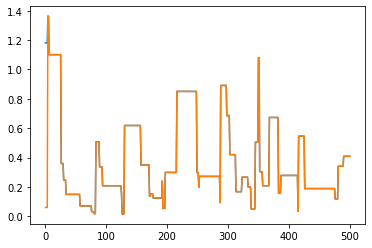
\includegraphics[width=6cm,height=3cm]{immagini_mario/k_chains}
			\end{center}
		\end{minipage}
		
		\vspace{0.2cm}
		
		\begin{minipage}{0.63\textwidth}
			\begin{center}
				{\scriptsize \textbf{Sampling histogram }}
				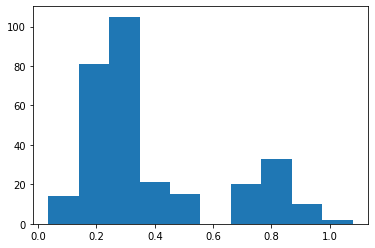
\includegraphics[width=6cm,height=3cm]{immagini_mario/k_hist}
			\end{center}
		\end{minipage}
	\end{center}
\end{frame}
\end{section}

\begin{section}{ABC + COUPLED MARKOV CHAINS}
\begin{frame}
	given $\theta =( a,b,g,k )$
	
	$ \theta_{1}^{(0)} \sim \mathcal{U}([0,10]^4)$
	
	$ \theta_{2}^{(0)} \sim \mathcal{U}([0,10]^4)$
	
	for j in (1,...,$n_{obs}$):
	\begin{itemize}
		\item $z^{(0,j)}(r) \sim \mathcal{N}(0,1)  $
		
		\item $ y_{1}^{(0,j)} \sim quantilefunction(z^{(0,j)}(r),\theta_{1}^{(0)})$
		
		\item compute $ s_{1}^{(0)} =S(y_{1}^{(0)})$
	\end{itemize}
	for j in (1,...,$n_{obs}$):
	
	\begin{itemize}
		\item $z^{(0,j)}(r) \sim \mathcal{N}(0,1)  $
		
		\item $ y_{2}^{(0,j)} \sim quantile function(z^{(0,j)}(r),theta_{2}^{(0)})$
		
		\item compute the summaries statistics:
		$ s_{2}^{(0)} =S(y_{2}^{(0)})$
	\end{itemize}
	
\end{frame}
\begin{frame}
	\frametitle{ABC + COUPLED MARKOV CHAIN for parameter a}
	Untill $Kh(\|s_{1}^{(0)} - s_{obs}\|)>0$:
	\begin{enumerate}
		\item Generate $\theta_{1}^{(0)} \sim \mathcal{U}([0,10]^4)$ from prior density.
		\item Generate $z_{1}^{(0)}(r) \sim \mathcal{N}(0,1)$
		\item Generate a sample of 1000 observations such that $y_{1} \sim quantile function(z_{1}^{(0)}(r),\theta_{1}^{0})$
		\item Compute $s_{1}^{(0)}=S(y_{1})$
		
	\end{enumerate}
	Untill $Kh(\|s_{2}^{(0)} - s_{obs}\|)>0$:
	\begin{enumerate}
		\item Generate $\theta_{2}^{(0)} \sim \mathcal{U}([0,10]^4)$ from prior density.
		\item Generate $z_{2}^{(0)}(r) \sim \mathcal{N}(0,1)$
		\item Generate a sample of 1000 observations such that $y_{2} \sim quantile function(z_{2}^{(0)}(r),theta_{2}^{(0)})$
		\item Compute $s_{2}^{(0)}=S(y_{2})$
	\end{enumerate}
	
\end{frame}
\begin{frame}
	\frametitle{ABC + COUPLED MARKOV CHAINS}
	for i in (1,...,M):
	\begin{enumerate}
		\item 	generate $\theta_{1}^{(i)},\theta_{2}^{(i)}$  from maximalcoupling$(\theta_{1}^{(i-1)},\theta_{2}^{(i-1)})$
		
		\begin{block}
			
			for j in (1,...,n):
			\begin{itemize}
				\item $z^{(i,j)}(r) \sim \mathcal{N}(0,1)$
				\item generate:
				$ y_{1}^{(ij)} \sim quantile function(z^{(i,j)}(r), \theta_{1}^{(i-1)})$
				$ y_{2}^{(ij)} \sim quantile function(z^{(i,j)}(r), \theta_{1}^{(i-1)})$
				
			\end{itemize}
		\end{block}
		\item Compute the summaries  $ s_{1}^{(i)} =S(y_{1}^{(i)})$ and $ s_{2}^{(i)} =S(y_{2}^{(i)})$
		
		
		\item acceptance:
		\begin{itemize}
			\item Accept $a_{1}^{(i)}$ with probability $\frac{Kh(\|s_{1}^{(i)}-s_{obs}\|)\pi(\theta_{1}^{(i)})}{Kh(\|s_{1}^{(i-1)}- s_{obs}\|)\pi(\theta_{1}^{(i-1)})} $   otherwise $a_{1}^{(i)}=\theta_{1}^{(i-1)}$
			
			\item Accept $a_{2}^{(i)}$ with probability $\frac{Kh(\|s_{2}^{(i)}-s_{obs}\|)\pi(\theta_{2}^{(i)})}{Kh(\|s_{2}^{(i-1)}-s_{obs}\|)\pi(\theta_{2}^{(i-1)})} $  otherwise $  \theta_{2}^{(i)}=\theta_{2}^{(i-1)}$
		\end{itemize}
	\end{enumerate}
\end{frame}

\begin{frame}
	\frametitle{Maximal coupling}
	given  $(\theta_{1}^{(i-1)}, \ \theta_{2}^{(i-1)})$
	
	set	$p( \cdot |\theta_{1}^{(i-1)})= \mathcal{N}(\theta_{1}^{(i-1)},0.1^2\mathbb{I})$ and $q( \cdot |\theta_{2}^{(i-1)})= \mathcal{N}(\theta_{2}^{(i-1)},0.1^2\mathbb{I})$
	\begin{enumerate}
		\item $ \theta_{1}' \sim p( \cdot |\theta_{1}^{(i-1)} ) $
		
		\item if $ w_{1}\sim \mathcal{U}((0, p(\theta'|\theta_{1}^{(i-1)}))) < q(\theta'|\theta_{2}^{(i-1)} ): \theta_{1}^{(i)}=\theta_{1}' \ and \ \theta_{2}^{(i)}= \theta_{1}'$
	\end{enumerate}
	otherwise until $ w_{2}\sim \mathcal{U}((0, q(\theta'|\theta_{2}^{(i-1)})) > p(\theta'|\theta_{1}^{(i-1)} )$:
	
	\begin{itemize}
		\item generate $ \theta_{2}' \sim q( \cdot |\theta_{2}^{(i-1)} ) $
		
		
	\end{itemize}
	and then set:   $ \ \theta_{1}^{(i)}=\theta_{1}' \ and \ \theta_{2}^{(i)}= \theta_{2}'$
	
	
\end{frame}



\begin{frame}
	\frametitle{Results: parameter a}
	
	\begin{center}
		{\scriptsize \textbf{Coupled chains}}
		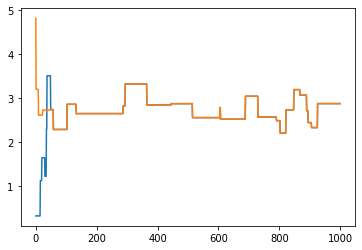
\includegraphics[width=6cm,height=3cm]{immagini_mario/a_all_chains}
		
	\end{center}
\end{frame}

\begin{frame}
	\frametitle{Results: parameter b}
	
	\begin{center}
		{\scriptsize \textbf{Coupled chains}}
		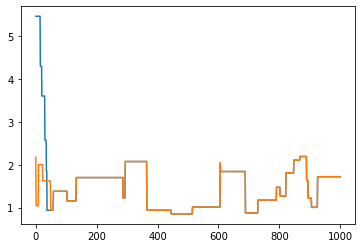
\includegraphics[width=6cm,height=3cm]{immagini_mario/b_all_chains}
	\end{center}
	
\end{frame}
\begin{frame}
	\frametitle{Results: parameter g}
	\begin{center}
		
		{\scriptsize \textbf{Coupled chains}}
		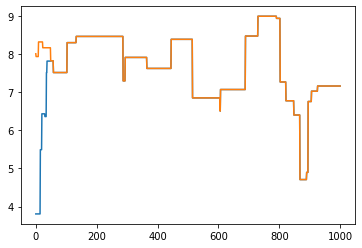
\includegraphics[width=6cm,height=3cm]{immagini_mario/g_all_chains}
		
		
	\end{center}
\end{frame}
\begin{frame}
	\frametitle{Results: parameter k}
	\begin{center}
		
		{\scriptsize \textbf{Coupled chains}}
		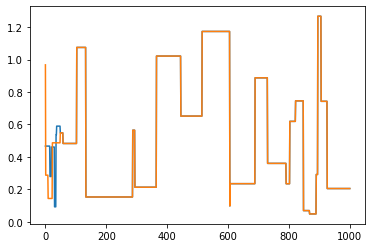
\includegraphics[width=6cm,height=3cm]{immagini_mario/k_all_chains}
		
		
		
	\end{center}
\end{frame}
\end{section}
\end{document}
